\documentclass[10pt]{article}
\usepackage{amsmath, amssymb, amsthm, mathtools, hyperref, multicol}
\usepackage[top=2cm, left = 2cm, right = 2cm, bottom = 3cm]{geometry}
\usepackage[pdftex]{graphicx}
\usepackage{asymptote,tikz}
\usepackage{fancyhdr}
\renewcommand{\bf}[1]{\textbf{#1}}
\newcommand{\N}{\mathbb{N}}
\pagestyle{fancy}
\rhead{}
\chead{\includegraphics[scale=0.17]{CMIMC-header-2017.png}}
\lhead{}
\setlength{\headheight}{43pt}
\rfoot{}
\cfoot{}
\lfoot{}
\newcommand{\proposed}[1]
{
\vspace{5pt}
\noindent\textit{Proposed by #1}
}
\newcommand{\eps}{\varepsilon}
\newcommand{\solution}
{
\vspace{5pt}
\noindent\textit{Solution.}\qquad
}
\DeclarePairedDelimiter\abs{\lvert}{\rvert}
\newcommand{\vp}{\varphi}
\newcommand{\ra}{\rightarrow}
\newcommand{\header}[1]
{
%\begin{center}
\section*{#1}
%\end{center}
}
\begin{document}\thispagestyle{empty}
\begin{center}

\vspace*{90pt}

\includegraphics[scale=0.3]{CMIMC-header-2017.png}

\includegraphics[scale=0.3]{CS-header.png}

\vspace{1.6in}

\includegraphics[scale=0.20]{Instruction-Header.png}
\noindent\rule{17.7cm}{2pt}
\end{center}

\vspace{10pt}

\begin{enumerate}
\large
\item Do not look at the test before the proctor starts the round.

\item This test consists of 10 short-answer problems to be solved in 60 minutes.
	Each question is worth one point.

\item Write your name, team name, and team ID on your answer sheet. Circle the
	subject of the test you are currently taking.

\item Write your answers in the corresponding boxes on the answer sheets.

\item No computational aids other than pencil/pen are permitted.

\item Answers must be reasonably simplified.

\item If you believe that the test contains an error, submit your protest in writing to Doherty 2302 by the end of lunch.
\end{enumerate}
\newpage

\newgeometry{margin=1.4cm, top = 0.7cm, bottom = 1.6cm}
\setlength\parindent{0pt}

\begin{center}
\Huge\textsf{\textbf{Computer Science Reference Sheet}}
\end{center}

\vspace{5pt}

\begin{multicols}{3}
\header{Psuedocode}
\subsection*{Code}
\noindent Code is written with line numbers indicated to the left.

\noindent Bold and caps lock indicates a special tag, including but not limited to \bf{TRUE}, \bf{FALSE}, \bf{IF}, \bf{ELSE IF}, \bf{FOR}, \bf{IN}, \bf{WHILE}, \bf{FUNCTION}, \bf{RETURN}, etc.

\subsection*{Variable Assignment}
\noindent [variable name] $\leftarrow$ [value]

\noindent This assigns [value] to [variable name].

\subsection*{Conditionals}
\noindent \bf{IF} [condition]

\noindent \qquad [code]

\noindent This executes [code] if [boolean condition] is true. \\
\\
\noindent \bf{ELSE IF} [condition]

\noindent \qquad[code]

\noindent This executes [code] if the previous boolean conditions are false and [boolean condition] is true.\\
\\
\noindent \bf{ELSE}

\noindent \,\,\, [code]

\noindent This executes [code] if all other boolean conditions are false.

\subsection*{Loops}

\bf{FOR} [variable] \bf{IN} [list]

\noindent \,\,\, [code]

\noindent This executes [code] iteratively for each value of [variable] in [list].\\
\\

\bf{WHILE}[conditional]

\noindent \,\,\, [code]

\noindent This executes [code] iteratively while [conditional] is true.

\subsection*{Functions}
\bf{FUNCTION} [name]([arguments])

This defines a function that takes in [arguments].\\
\\
\bf{RETURN} [value]

This causes the function to immediately return [value].

\header{Big $O$, $\Omega$, $\Theta$}

A function $f(n)$ is said to be $O(g(n))$ if there exists a constant $c>0$ such that $f(n)<c\cdot g(n)$ for all sufficiently large $n$.

A function $f(n)$ is said to be $\Omega(g(n))$ if there exists a constant $c>0$ such that $f(n)<c\cdot g(n)$ for all sufficiently large $n$.

A function $f(n)$ is said to be $\Theta(g(n))$ if it is both $O(g(n))$ and $\Theta(g(n))$.

\header{Data Structures}

\subsection*{Arrays}

A collection of elements accessed by indices.

\begin{center}
\includegraphics[scale=0.6]{array.PNG}
\end{center}

\vspace{-15pt}

\subsection*{Lists}

A sequence of elements, each pointing to the next element and the last one pointing to null.

\begin{center}
\includegraphics[scale=0.6]{list.png}
\end{center}

\vspace{-15pt}

\subsection*{Stacks}

A set with a top and bottom where elements are added to the top and removed from the top (first-in first-out).

\begin{center}
\includegraphics[scale=0.6]{stack.png}
\end{center}

\vspace{-15pt}

\subsection*{Queues}

A set with a front and back where elements are added to the back and removed from the front (first-in last-out).

\begin{center}
\includegraphics[scale=0.6]{queue.png}
\end{center}

\header{Graph Theory}

A \textit{graph} is a set of vertices $V$ and a set of edges $E\subseteq V\times V$.  Two vertices $V_1$ and $V_2$ are \textit{adjacent} (denoted $V_1\sim V_2$) iff there is an edge connecting them.

The \textit{neighbors} of a vertex are all vertices adjacent to it.  The \textit{degree} of a vertex is its number of neighbors.

A \textit{path} is a sequence of vertices $\{v_j\}_{j=0}^k$ such that $v_i\sim v_{i+1}$ for all $i$ and such that no $v_j$ is visited twice.  A cycle is like a path but with $v_0\sim v_k$.  If a graph contains no cycles, it is said to be a \textit{tree}.

\begin{center}
\includegraphics[scale=0.6]{tree.png}
\end{center}

A graph is \textit{connected} if for every two vertices there exists a path from one to the other.  Otherwise, it is \textit{disconnected}.  The \textit{distance} between any two vertices in a connected graph is the length of the shortest path from one to the other.

\header{Logic}

A \textit{boolean function} is a function $f:\{0,1\}^n\to\{0,1\}$.  We can write its \textit{truth table} by listing all possible inputs with its outputs.

The three main boolean operators are \bf{NOT} ($\neg$), \bf{AND} ($\wedge$), \bf{OR} ($\vee$), and \bf{XOR} ($\oplus$).  Their truth tables are listed below:

\begin{center}
\includegraphics[scale=0.6]{truth.png}
\end{center}

\header{Strings}

An \textit{alphabet} is any finite set of symbols.  We usually denote an alphabet by $\Sigma$.

A \textit{string} is a sequence of elements from an alphabet.  We denote the empty string by $\eps$.

The \textit{length} of a string is the length of the sequence it represents.  Length is denoted by $|\cdot|$.

For a string $s=s_0s_1s_2\ldots$, the substring starting at $i$ ending at $j$, denoted $s[i,j)$, is the substring $s_is_{i+1}\ldots s_j$.  This is only well-defined when $0\leq i\leq j-1$, but we also define the substring to be empty if $i=j$.

The concatenation of two strings $A$ and $B$ is the string $AB$.  The concatenation of $n$ copies of the string $s$ is denoted by $s^n$, where $s^0=\eps$.
\end{multicols}

\newpage

\restoregeometry
\setlength\parindent{1.5em}

\begin{center}
\huge\textbf{Computer Science}\normalsize

\vspace{3pt}
\end{center}

\begin{enumerate}

\item What is the minimum number of times you have to take your pencil off the paper to draw the following figure (the dots are for decoration)? You must lift your pencil off the paper after you're done, and this is included in the number of times you take your pencil off the paper. You're not allowed to draw over an edge twice. 

\begin{center}
\begin{tikzpicture}
\foreach \x in {0,...,4}{
\draw (\x,\x/2*0.75) -- (5,\x*0.75-2.5*0.75);
\draw (\x,-\x/2*0.75) -- (5,2.5*0.75-\x*0.75);
}
\foreach \x in {0,...,5}{
\foreach \y in {0,...,\x}{
\draw [fill=black] (\x,\y*0.75-\x*0.5*0.75) circle (0.1);
}
}
\end{tikzpicture}
\end{center}






\item We are given the following function $f$, which takes a list of integers and outputs another list of integers.  (Note that here the list is zero-indexed.)

\begin{tabular}{l}
1: \textbf{FUNCTION} $f(A)$ \\
2: $\quad$ \textbf{FOR} $i=1,\ldots, \operatorname{length}(A)-1$: \\
3: $\quad\quad$ $A[i]\leftarrow A[A[i]]$ \\
4: $\quad\quad$ $A[0]\leftarrow A[0]-1$ \\
5: $\quad$ \textbf{RETURN} $A$
\end{tabular}

\par Suppose the list $B$ is equal to $[0,1,2,8,2,0,1,7,0]$.  In how many entries do $B$ and $f(B)$ differ?





\item In the following list of numbers (given in their binary representations), each number appears an even number of times, except for one number that appears exactly three times. Find the number that appears exactly three times. Leave the answer in its binary representation.

\begin{center}
\begin{tabular}{cccccc}
010111 & 000001 & 100000 & 011000 & 110101 & 100001 \\
010100 & 011111 & 111001 & 010001 & 010100 & 101100 \\
010001 & 011011 & 011111 & 011011 & 100000 & 000001 \\
110011 & 001000 & 111101 & 100001 & 101100 & 110011 \\
111111 & 011000 & 001000 & 101000 & 111111 & 101000 \\
010111 & 100011 & 111001 & 100011 & 110101 & 011111 \\
100000 & 010100 & 010001 & 101100 & 010111 & 011011 \\
011000 & 111101 & 111111 & 100001 & 101000 & 100011 \\
011011 & 010111 & 110011 & 111111 & 000001 & 010001 \\
101000 & 111001 & 010100 & 110101 & 011000 & 110101 \\
001000 & 000001 & 100000 & 111101 & 100011 & 001000 \\
111001 & 110011 & 100001 & 011111 & 101100 
\end{tabular}
\end{center}




\item How many complete directed graphs with vertex set $V=\{1,2,3,4,5,6\}$ contain no $3$-cycles?

\par A graph is \textit{directed} if all edges have a direction (e.g. from $u$ to $v$ rather than between $u$ and $v$), and \textit{complete} if every pair of vertices has an edge between them. Further, a \textit{3-cycle} in a directed graph is a triple $(u,v,w)$ of vertices such that there are edges from $u$ to $v$, $v$ to $w$, and $w$ to $u$.


\newpage
\item Given a list $A$ of $n$ real numbers, the following algorithm, known as \textit{insertion sort}, sorts the elements of $A$ from least to greatest.

	\begin{tabular}{l}
		1: \textbf{FUNCTION} $IS(A)$ \\
		2: $\quad$ \textbf{FOR} $i=0,\ldots, n-1$: \\
		3: $\quad\quad$ $j \leftarrow i$\\
		4: $\quad\quad$ \textbf{WHILE} $j>0$ \& $A[j-1]>A[j]:$\\
		5: $\quad\quad\quad$ \textbf{SWAP} $A[j], A[j-1]$\\
		6: $\quad\quad\quad$ $j \leftarrow j-1$\\
		7: \textbf{RETURN} $A$
	\end{tabular}

	As $A$ ranges over all permutations of $\{1, 2, \ldots, n\}$, let $f(n)$ denote the expected number of comparisons (i.e., checking which of two elements is greater) that need to be made when sorting $A$ with insertion sort. Evaluate $f(13) - f(12)$.




\item Define a self-balanced tree to be a tree such that for any node, the size of the left subtree is within 1 of the size of the right subtree. How many balanced trees are there of size 2046?




\item You are presented with a mystery function $f:\mathbb N^2\to\mathbb N$ which is known to satisfy \[f(x+1,y)>f(x,y)\quad\text{and}\quad f(x,y+1)>f(x,y)\] for all $(x,y)\in\mathbb N^2$. I will tell you the value of $f(x,y)$ for \$1. What's the minimum cost, in dollars, that it takes to compute the $19$th smallest element of $\{f(x,y)\mid(x,y)\in\mathbb N^2\}$? Here, $\mathbb N=\{1,2,3,\dots\}$ denotes the set of positive integers.





\item We have a collection of $1720$ balls, half of which are black and half of which are white, aligned in a straight line. Our task is to make the balls alternating in color along the line. The following greedy algorithm accomplishes that task for $2n$ balls:

\iffalse
\begin{verbatim}
for i = 2, 3, ..., 2n
  if balls i-1 and i have the same color
    j <- smallest index > i for which balls i-1 and j have different colors
    swap balls i and j
\end{verbatim}
\fi

\begin{tabular}{l}
1: \textbf{FOR} $i$ \textbf{IN} $[2,3,\dots,2n]$ \\
2: $\quad$ \textbf{IF} balls $i-1$ and $i$ have the same color: \\
3: $\quad\quad$ $j\gets$ smallest index greater than $i$ for which balls $i-1$ and $j$ have different colors \\
4: $\quad\quad$ swap balls $i$ and $j$
\end{tabular}

Given a configuration $C$ of our $1720$ balls, let $\hat{\sigma}(C)$ denote the number of swaps the greedy algorithm takes, and let $\sigma(C)$ denote the minimum number of swaps actually necessary to perform the task. Find the maximum value over all configurations $C$ of $\hat{\sigma}(C)-\sigma(C)$.





\item Alice thinks of an integer $1 \le n \le 2048$. Bob asks $k$ true or false questions about Alice's integer; Alice then answers each of the questions, but she may lie on at most one question. What is the minimum value of $k$ for which Bob can guarantee he knows Alice's integer after she answers?





\item How many distinct spanning trees does the graph below have? Recall that a \emph{spanning tree} of a graph $G$ is a subgraph of $G$ that is a tree and containing all the vertices of $G$.

\begin{center}
\begin{tikzpicture}[scale=1.5]
\draw (0.,0.)-- (0.,2.);
\draw (0.,2.)-- (1.,0.);
\draw (1.,0.)-- (1.,2.);
\draw (1.,2.)-- (2.,0.);
\draw (2.,0.)-- (2.,2.);
\draw (2.,2.)-- (3.,0.);
\draw (3.,0.)-- (3.,2.);
\draw (3.,2.)-- (4.,0.);
\draw (4.,0.)-- (4.,2.);
\draw (4.,2.)-- (5.,0.);
\draw (5.,0.)-- (5.,2.);
\draw (5.,2.)-- (4.,0.);
\draw (0.,2.)-- (2.,0.);
\draw (0.,2.)-- (3.,0.);
\draw (0.,2.)-- (4.,0.);
\draw (0.,2.)-- (5.,0.);
\draw (1.,2.)-- (0.,0.);
\draw (1.,2.)-- (3.,0.);
\draw (1.,2.)-- (4.,0.);
\draw (1.,2.)-- (5.,0.);
\draw (2.,2.)-- (0.,0.);
\draw (2.,2.)-- (1.,0.);
\draw (2.,2.)-- (4.,0.);
\draw (2.,2.)-- (5.,0.);
\draw (3.,2.)-- (0.,0.);
\draw (3.,2.)-- (1.,0.);
\draw (3.,2.)-- (2.,0.);
\draw (3.,2.)-- (5.,0.);
\draw (4.,2.)-- (0.,0.);
\draw (4.,2.)-- (1.,0.);
\draw (4.,2.)-- (2.,0.);
\draw (4.,2.)-- (3.,0.);
\draw (5.,2.)-- (0.,0.);
\draw (5.,2.)-- (1.,0.);
\draw (5.,2.)-- (2.,0.);
\draw (5.,2.)-- (3.,0.);
\begin{scriptsize}
	\draw [fill=black] (0.,0.) circle (1.5pt);
	\draw[color=black] (0.,-0.25) node {$b_{1}$};
	\draw [fill=black] (1.,0.) circle (1.5pt);
	\draw[color=black] (1.,-0.25) node {$b_{2}$};
	\draw [fill=black] (2.,0.) circle (1.5pt);
	\draw[color=black] (2.,-0.25) node {$b_{3}$};
	\draw [fill=black] (3.,0.) circle (1.5pt);
	\draw[color=black] (3,-0.25) node {$b_{4}$};
	\draw [fill=black] (4.,0.) circle (1.5pt);
	\draw[color=black] (4.,-0.25) node {$b_{5}$};
	\draw [fill=black] (5.,0.) circle (1.5pt);
	\draw[color=black] (5.,-0.25) node {$b_{6}$};
	\draw [fill=black] (0.,2.) circle (1.5pt);
	\draw[color=black] (0.,2.25) node {$a_{1}$};
	\draw [fill=black] (1.,2.) circle (1.5pt);
	\draw[color=black] (1.,2.25) node {$a_{2}$};
	\draw [fill=black] (2.,2.) circle (1.5pt);
	\draw[color=black] (2.,2.25) node {$a_{3}$};
	\draw [fill=black] (3.,2.) circle (1.5pt);
	\draw[color=black] (3.,2.25) node {$a_{4}$};
	\draw [fill=black] (4.,2.) circle (1.5pt);
	\draw[color=black] (4.,2.25) node {$a_{5}$};
	\draw [fill=black] (5.,2.) circle (1.5pt);
	\draw[color=black] (5.,2.25) node {$a_{6}$};
\end{scriptsize}
\end{tikzpicture}
\end{center}

\end{enumerate}


\end{document}
